\def\baselinestretch{1}
%\chapter{CONCLUSIONS AND DISCUSSION} \label{chap:conclusion}
\chapter{\MakeUppercase{\ChapterTitleSeven}} \label{chap:conclusion}
    \minitoc
    
    %\newpage
\begin{center}
	%\emph{Abstract of chapter \ref{chap:conclusion}}
	\emph{Abstract}
\end{center}

    This chapter offers a comprehensive synthesis of findings from the study of Supersoft X-ray Sources (SSS), focusing on their physical interpretation, implications, and future research directions. The chapter highlights the diversity of SSS types in both the Milky Way and the Large Magellanic Cloud, noting differences in spectral features, luminosity, and X-ray characteristics that suggest varying environmental and intrinsic properties. The detection of absorption edges in Milky Way SSS versus their absence in LMC counterparts implies significant interstellar medium absorption effects. Higher luminosity in sources like RX J0925.7-4758 is linked to elevated mass accretion rates, which are also associated with distinctive spectral features. The application of a multi-component non-local thermodynamic equilibrium (NLTE) model effectively captures the continuum spectra, while low-frequency modulations suggest complex mechanisms such as orbital variations and stellar pulsations. These findings provide insight into the evolutionary pathways of SSS, influenced by factors like companion type, accretion processes, and magnetic field strength. The successful use of the Lomb-Scargle periodogram underscores its value in characterising periodic variability in SSS. Looking forward, the chapter calls for extended spectral analysis, broader sample studies, high-resolution timing observations, enhanced theoretical modelling, and cross-instrument data comparisons to deepen our understanding of these enigmatic systems.
    
    \setcounter{footnote}{\value{footnotecount}}

    \newpage
    \section{\MakeUppercase{Physical Interpretation}}
    \begin{itemize}
    	\item \textit{Diverse SSS Types}: We have assembled a unique dataset encompassing a variety of SSS types (X-ray binaries, cataclysmic variables, and a symbiotic system) from both the Milky Way and the Large Magellanic Cloud, providing a diverse sample for our investigation.
    	%The dataset includes a variety of SSS types (X-ray binaries, cataclysmic variables, and a symbiotic system) from both the Milky Way and the Large Magellanic Cloud, providing a broad spectrum of physical conditions for analysis.
    	
    	\item \textit{Spectral Features}: Our analysis has revealed that the SSS in the Milky Way exhibit discernible absorption edges, suggesting differences in local environmental conditions or interstellar absorption. These findings are novel and contribute to our understanding of the interstellar medium in different galactic environments.
    	%Analysis reveals that the SSS in the Milky Way exhibit discernible absorption edges, indicating higher localised absorption. In contrast, the absence of clear absorption edges in LMC SSS suggests these features may be diluted due to greater interstellar medium absorption along the line of sight.
    	
    	\item \textit{Luminosity and Distance}: We have discovered that RX J0925.7-4758, despite its greater distance, exhibits significantly higher luminosity than RS Oph. This implies a higher mass accretion rate in RX J0925.7-4758, which is a novel finding and provides valuable insights into the accretion processes in SSS.
    	%RX J0925.7-4758, despite being farther than RS Oph, exhibits significantly higher count rates, implying it is intrinsically more luminous. This suggests a higher mass accretion rate in RX J0925.7-4758 compared to RS Oph.
    	
    	\item \textit{Softer X-ray Characteristics}: Our analysis has identified softer X-ray emissions from certain SSS (namely CAL 83, RX J0527.8-6954, and RX J0019.8+2156), indicating differences in their effective temperatures and accretion processes. These findings are new and contribute to our understanding of the diversity among SSS.
    	%SSS like CAL 83, RX J0527.8-6954, and RX J0019.8+2156 show softer X-ray emissions compared to RX J0925.7-4758 and RS Oph, indicating differences in their effective temperatures and possibly the nature of their accretion processes.
    	
    	\item \textit{Spectral Modelling}: We have successfully employed a multi-component NLTE model to accurately capture the continuum spectrum of RX J0925.7-4758. This novel approach demonstrates the potential of similar modeling techniques to constrain the stellar parameters of other SSS, providing valuable insights into their physical properties.
    	%The use of a multi-component NLTE model effectively captures the continuum spectrum of RX J0925.7-4758, suggesting similar modelling can constrain the stellar parameters of other SSS.
    \end{itemize}
    
    \section{\MakeUppercase{Implications}}
    	\begin{itemize}
    		\item \textit{Galactic vs. Extragalactic SSS}: The absence of clear absorption edges in LMC SSS, compared to Milky Way SSS, suggests differences in local environmental conditions or the impact of interstellar absorption, potentially offering insights into the ISM properties of different galaxies.
    		
    		\item \textit{Mass Accretion Insights}: Higher luminosity and the presence of multiple absorption edges in RX J0925.7-4758 highlight the role of high accretion rates in shaping the observed spectral characteristics, which could help model the evolution of such systems.
    		
    		\item \textit{Periodic Variability}: The detection of low-frequency modulations in RX J0925.7-4758 points to possible mechanisms such as orbital variations, accretion dynamics, or stellar pulsations, which can influence the emission properties of SSS.
    		
    		\item \textit{Evolutionary Pathways}: Differences in spectral hardness and variability between the SSS suggest diverse evolutionary pathways, potentially influenced by factors like companion type, accretion rate, and magnetic field strength.
    		
    		\item \textit{Diagnostic Tools}: The successful application of the Lomb-Scargle periodogram to identify periodic signals reinforces its utility in the timing analysis of variable X-ray sources, providing a robust method for detecting and characterising periodicity.
    	\end{itemize}
    
    \section{\MakeUppercase{Future Scope}}
    	\begin{itemize}
    		\item \textit{Extended Spectral Analysis}: Further analysis of high-resolution spectra from instruments like RGS could help identify more subtle spectral features, enhancing our understanding of the atmospheres and environments of these SSS.
    		
    		\item \textit{Broader Sample Studies}: Expanding the dataset to include more SSS from different galaxies could improve statistical robustness and help uncover universal properties or distinct characteristics linked to specific galactic environments.
    		
    		\item \textit{Upgrades to Line-identification Code}: The Python code for line-identification, in its current version, is limited to RGS fluxed spectra from XMM-Newton. While it is not planned to support binned spectra, future versions will likely include support for EPIC MOS and PN data. The code currently produces velocity profiles for only the first three Lyman lines of specific ions. Future updates aim to expand this to include any ground transition of any ion and introduce filtering based on transition probability to reduce line clutter.
    		
    		\item \textit{High-Resolution Timing Studies}: More precise timing observations using advanced instruments can help distinguish between intrinsic variability and observational artefacts, leading to a clearer understanding of the periodic phenomena in SSS. Relevant examples are the \textit{Resolve} and \textit{Xtend} instruments on-board the \textit{XRISM} observatory, launched by JAXA and NASA on 6 September 2023 \cite{tashiro2022xrism}. While Resolve is for high-resolution spectroscopy, Xtend is for wide-field imaging; both being designed to operate over the full range of SSS energies.
    		
    		\item \textit{Theoretical Modelling}: Development of more sophisticated NLTE models incorporating complex absorption and emission processes could provide better fits to observed spectra and yield more accurate stellar parameters.
    		
    		\item \textit{Cross-Instrument Comparisons}: Combining data from different observatories like NICER, XMM-Newton, and future missions could refine our understanding of SSS variability and emission mechanisms, leveraging each instrument's strengths.
    		
    		\item \textit{Study of Circumstellar Material}: Investigating the role of circumstellar material, such as stellar winds or disks, in shaping the observed X-ray characteristics could provide insights into the accretion dynamics and evolution of these systems.
    	\end{itemize}

\includepdf[pages={11}]{bibliography.pdf}

	\setcounter{footnotecount}{\value{footnote}}